\documentclass[tikz,border=15pt]{standalone}
\usetikzlibrary{matrix, arrows.meta, positioning, calc, fit, backgrounds}
\usepackage{amssymb, amsmath}

\begin{document}
	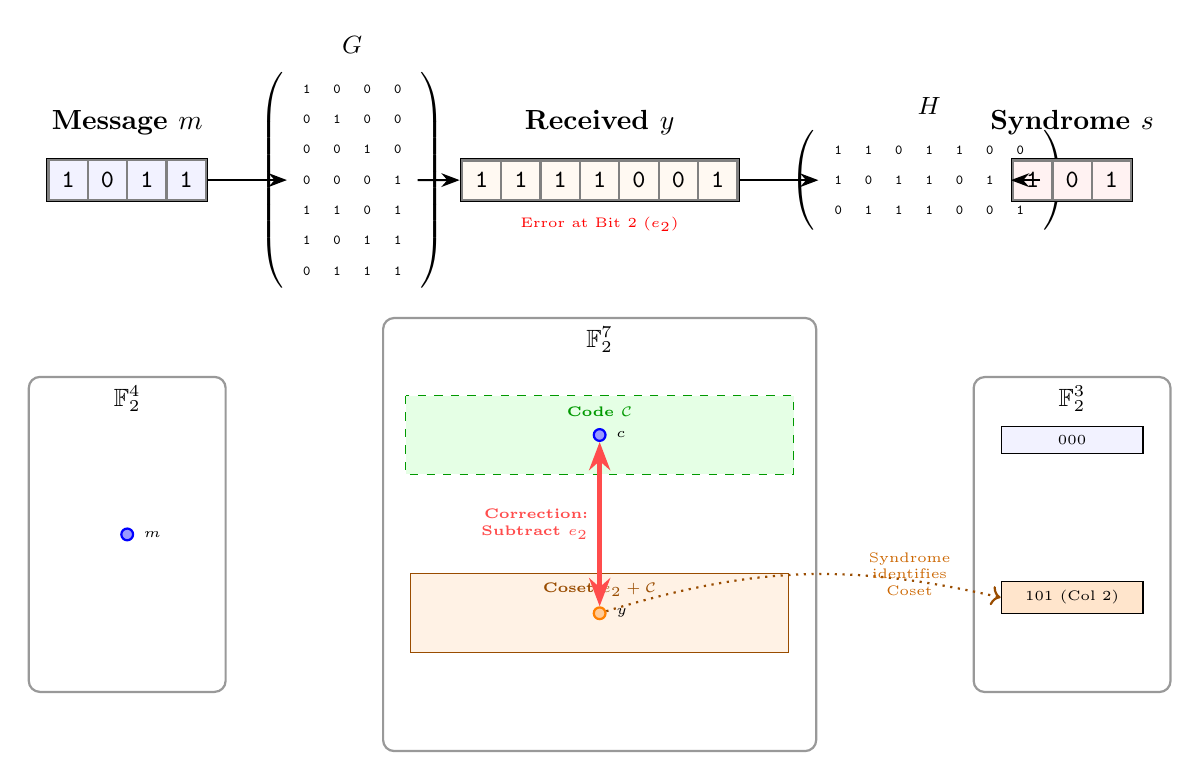
\begin{tikzpicture}[
		font=\sffamily,
		% Register styles
		bitvector/.style={matrix of nodes, nodes={draw=black!50, minimum size=5mm, anchor=center, font=\ttfamily\small}, column sep=-\pgflinewidth, row sep=-\pgflinewidth, inner sep=0pt, draw=black, thick},
		% Transformation Matrix styles
		opmatrix/.style={matrix of nodes, nodes={font=\ttfamily\tiny, minimum size=3.5mm, anchor=center}, left delimiter=(, right delimiter=), column sep=1pt, row sep=1pt, inner sep=2pt},
		% Subspace/Memory styles
		membox/.style={draw=black!40, thick, rounded corners, fill=white},
		point/.style={fill=blue!40, draw=blue, thick, circle, inner sep=1.5pt}
		]
		
		% --- TOP ROW: ALGEBRAIC PIPELINE ---
		\node[font=\bfseries] (T1) at (0,0) {Message $m$};
		\matrix (m_reg) [bitvector, below=5pt of T1, fill=blue!5] { 1 & 0 & 1 & 1 \\ };
		
		\matrix (G_mat) [opmatrix, right=1cm of m_reg] {
			1 & 0 & 0 & 0 \\ 0 & 1 & 0 & 0 \\ 0 & 0 & 1 & 0 \\ 0 & 0 & 0 & 1 \\
			1 & 1 & 0 & 1 \\ 1 & 0 & 1 & 1 \\ 0 & 1 & 1 & 1 \\
		};
		\node[above=2pt of G_mat, font=\itshape\small] {$G$};
		
		\node[font=\bfseries] (T2) at (6,0) {Received $y$};
		\matrix (c_reg) [bitvector, below=5pt of T2, fill=orange!5] { 1 & 1 & 1 & 1 & 0 & 0 & 1 \\ };
		\node[below=2pt of c_reg, font=\tiny, red] {Error at Bit 2 ($e_2$)};
		
		\matrix (H_mat) [opmatrix, right=1cm of c_reg] {
			1 & 1 & 0 & 1 & 1 & 0 & 0 \\ 1 & 0 & 1 & 1 & 0 & 1 & 0 \\ 0 & 1 & 1 & 1 & 0 & 0 & 1 \\
		};
		\node[above=2pt of H_mat, font=\itshape\small] {$H$};
		
		\node[font=\bfseries] (T3) at (12,0) {Syndrome $s$};
		\matrix (s_reg) [bitvector, below=5pt of T3, fill=red!5] { 1 & 0 & 1 \\ };
		
		\draw[-Stealth, thick] (m_reg) -- (G_mat);
		\draw[-Stealth, thick] (G_mat) -- (c_reg);
		\draw[-Stealth, thick] (c_reg) -- (H_mat);
		\draw[-Stealth, thick] (H_mat) -- (s_reg);
		
		% --- BOTTOM ROW: GEOMETRIC SPACES ---
		\coordinate (offset) at (0,-5.5);
		
		% A. Message Space
		\node[membox, minimum width=2.5cm, minimum height=4cm] (Space_m) at ($(m_reg) + (0,-4.5)$) {};
		\node[anchor=north, font=\small\bfseries] at (Space_m.north) {$\mathbb{F}_2^4$};
		\node[point, label=right:{\tiny $m$}] (p_m) at (Space_m.center) {};
		
		% B. Ambient Space F2^7
		\node[membox, minimum width=5.5cm, minimum height=5.5cm] (Space_c) at ($(c_reg) + (0,-4.5)$) {};
		\node[anchor=north, font=\small\bfseries] at (Space_c.north) {$\mathbb{F}_2^7$};
		
		% Codeword Subspace
		\draw[fill=green!10, draw=green!60!black, dashed] 
		($(Space_c.north west) + (0.3,-1.0)$) rectangle ($(Space_c.north east) + (-0.3,-2.0)$);
		\node[font=\tiny\bfseries, green!60!black] at ($(Space_c.north) + (0,-1.2)$) {Code $\mathcal{C}$};
		\node[point, label=right:{\tiny $c$}] (p_c) at ($(Space_c.north) + (0,-1.5)$) {};
		
		% Error Coset
		\draw[fill=orange!10, draw=orange!60!black] 
		($(Space_c.center) + (-2.4, -0.5)$) rectangle ($(Space_c.center) + (2.4, -1.5)$);
		\node[font=\tiny\bfseries, orange!60!black] at ($(Space_c.center) + (0,-0.7)$) {Coset $e_2 + \mathcal{C}$};
		\node[point, label=right:{\tiny $y$}, fill=orange!40, draw=orange] (p_y) at ($(Space_c.center) + (0,-1)$) {};
		
		% DECODING JUMP ARROW
		\draw[->, ultra thick, red!70, Stealth-Stealth] (p_y) -- (p_c) 
		node[midway, left, font=\tiny\bfseries, align=right] {Correction:\\Subtract $e_2$};
		
		% C. Syndrome Space F2^3
		\node[membox, minimum width=2.5cm, minimum height=4cm] (Space_s) at ($(s_reg) + (0,-4.5)$) {};
		\node[anchor=north, font=\small\bfseries] at (Space_s.north) {$\mathbb{F}_2^3$};
		
		\node[draw, fill=blue!5, minimum width=1.8cm, font=\tiny] (syn0) at ($(Space_s.center) + (0, 1.2)$) {$000$};
		\node[draw, fill=orange!20, minimum width=1.8cm, font=\tiny] (synE) at ($(Space_s.center) + (0, -0.8)$) {$101$ (Col 2)};
		
		% Cross-space Logic
		\draw[->, orange!60!black, dotted, thick] (p_y) to[bend left=15] (synE.west);
		\node[font=\tiny, orange!80!black, align=center] at ($(Space_s.west) + (-0.8, -0.5)$) {Syndrome\\identifies\\Coset};
		
	\end{tikzpicture}
\end{document}